% Native editable composition from verified, unchanged IDE images.
\par
\begin{figure}[htbp]
  \centering
  \sbox0{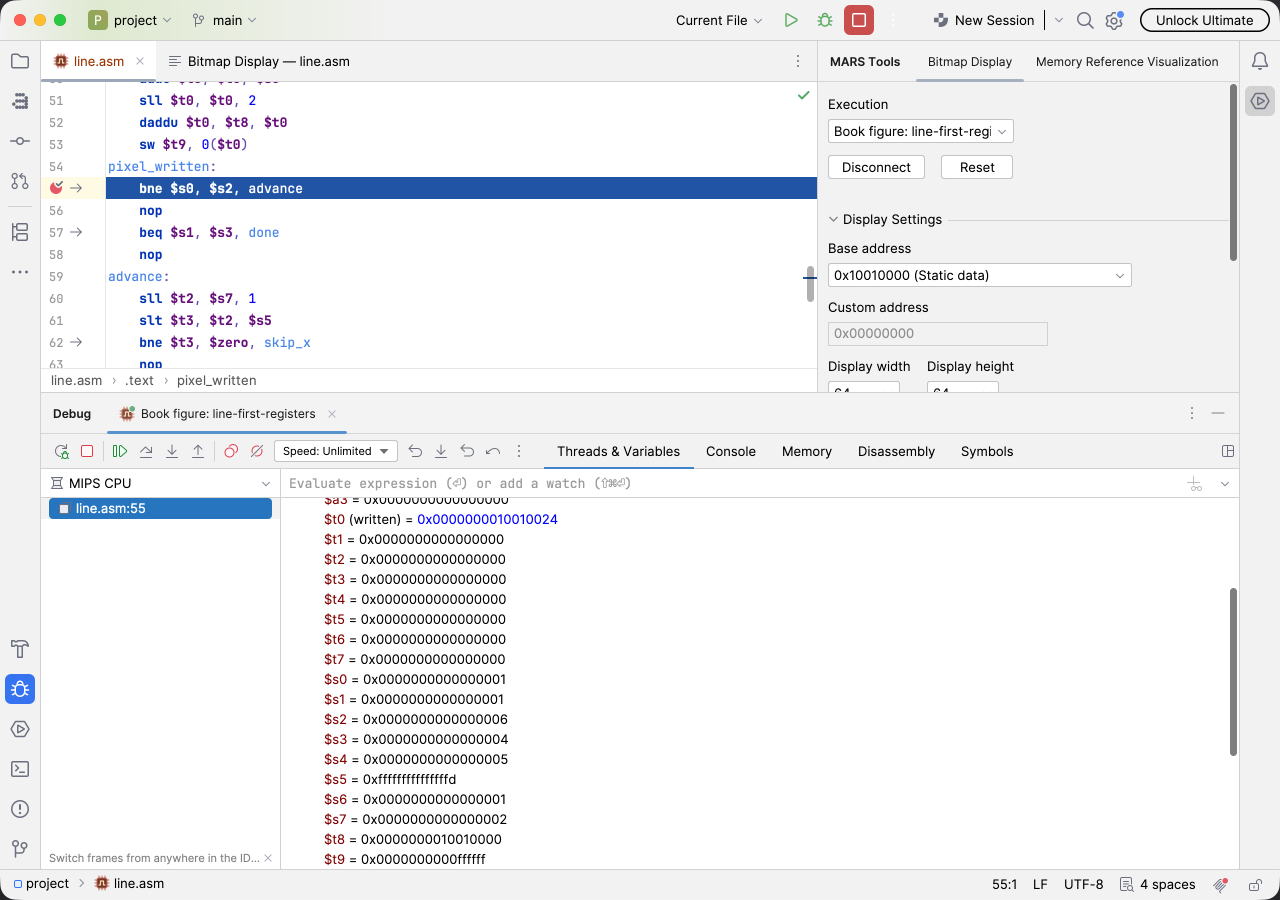
\includegraphics[artifact]{packages/007-bresenham-line/captures/f01-first/registers.png}}
  \sbox2{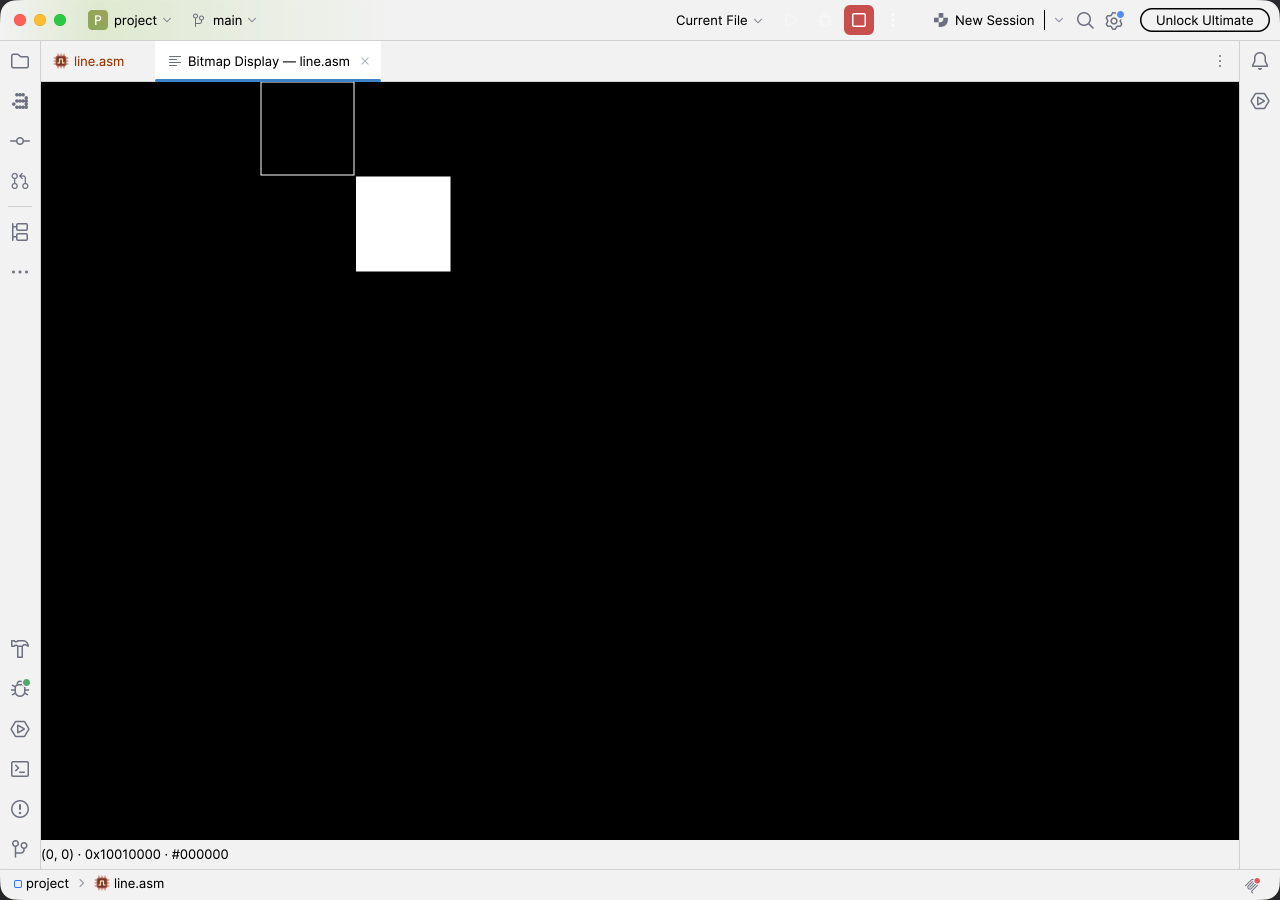
\includegraphics[artifact]{packages/007-bresenham-line/captures/f01-first/bitmap.png}}
  \edef\MARSfirstsourceLeft{\the\dimexpr0.036718750\wd0\relax}
  \edef\MARSfirstsourceBottom{\the\dimexpr0.774444444\ht0\relax}
  \edef\MARSfirstsourceRight{\the\dimexpr0.611718750\wd0\relax}
  \edef\MARSfirstsourceTop{\the\dimexpr0.147777778\ht0\relax}
  \edef\MARSfirststateLeft{\the\dimexpr0.246093750\wd0\relax}
  \edef\MARSfirststateBottom{\the\dimexpr0.075555556\ht0\relax}
  \edef\MARSfirststateRight{\the\dimexpr0.597656250\wd0\relax}
  \edef\MARSfirststateTop{\the\dimexpr0.740000000\ht0\relax}
  \edef\MARSfirstplotLeft{\the\dimexpr0.203906250\wd2\relax}
  \edef\MARSfirstplotBottom{\the\dimexpr0.066666667\ht2\relax}
  \edef\MARSfirstplotRight{\the\dimexpr0.203906250\wd2\relax}
  \edef\MARSfirstplotTop{\the\dimexpr0.091111111\ht2\relax}
  \begin{tikzpicture}[alt={Three annotated details at the first pixel written boundary. The next source instruction tests x against the endpoint. Registers s0 and s1 contain one and one, and s7 contains two. The original eight by eight bitmap has only cell one one white. Added coordinate labels outside the image number columns and rows zero through seven.}]
    \node[anchor=north west,inner sep=0,font=\small\bfseries] (source-title) at (6mm,0) {Stop after the store, before the endpoint test};
    \node[anchor=north west,inner sep=0] (source) at ([yshift=-1mm]source-title.south west) {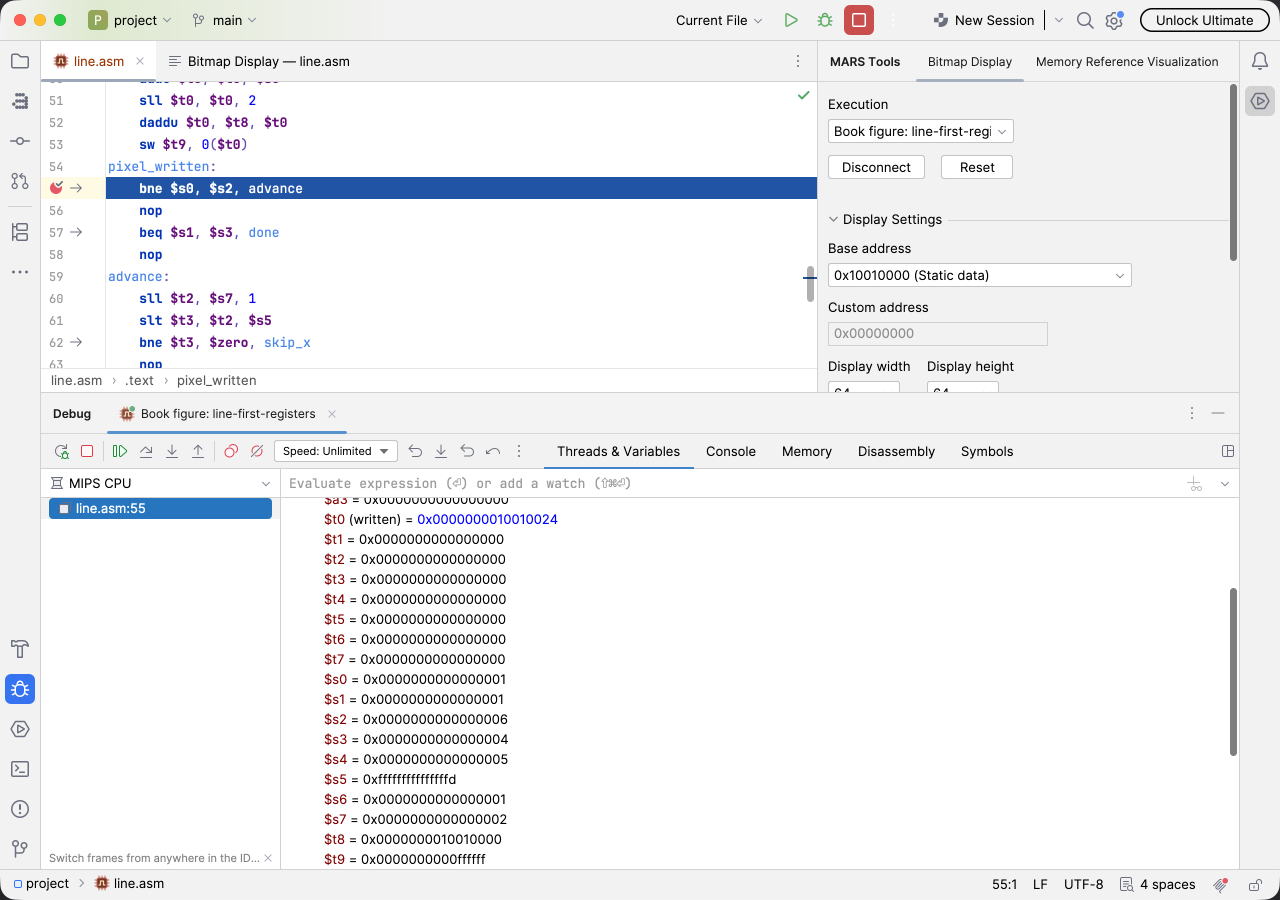
\includegraphics[width=0.7\linewidth,artifact,trim={\MARSfirstsourceLeft{} \MARSfirstsourceBottom{} \MARSfirstsourceRight{} \MARSfirstsourceTop{}},clip]{packages/007-bresenham-line/captures/f01-first/registers.png}};
    \begin{scope}[shift={(source.south west)},x={($(source.south east)-(source.south west)$)},y={($(source.north west)-(source.south west)$)}]
      \draw[black,line width=0.7pt] (0.135555556,0.057142857) rectangle (0.568888889,0.371428571);
      \node[draw=black,fill=white,circle,inner sep=1.5pt,font=\footnotesize] at ($(0.135555556,0.371428571)+(-3mm,0)$) {1};
    \end{scope}
    \node[anchor=north west,inner sep=0,font=\small\bfseries] (state-title) at ([yshift=-2mm]source.south west) {The first coordinate and error};
    \node[anchor=north west,inner sep=0] (state) at ([yshift=-1mm]state-title.south west) {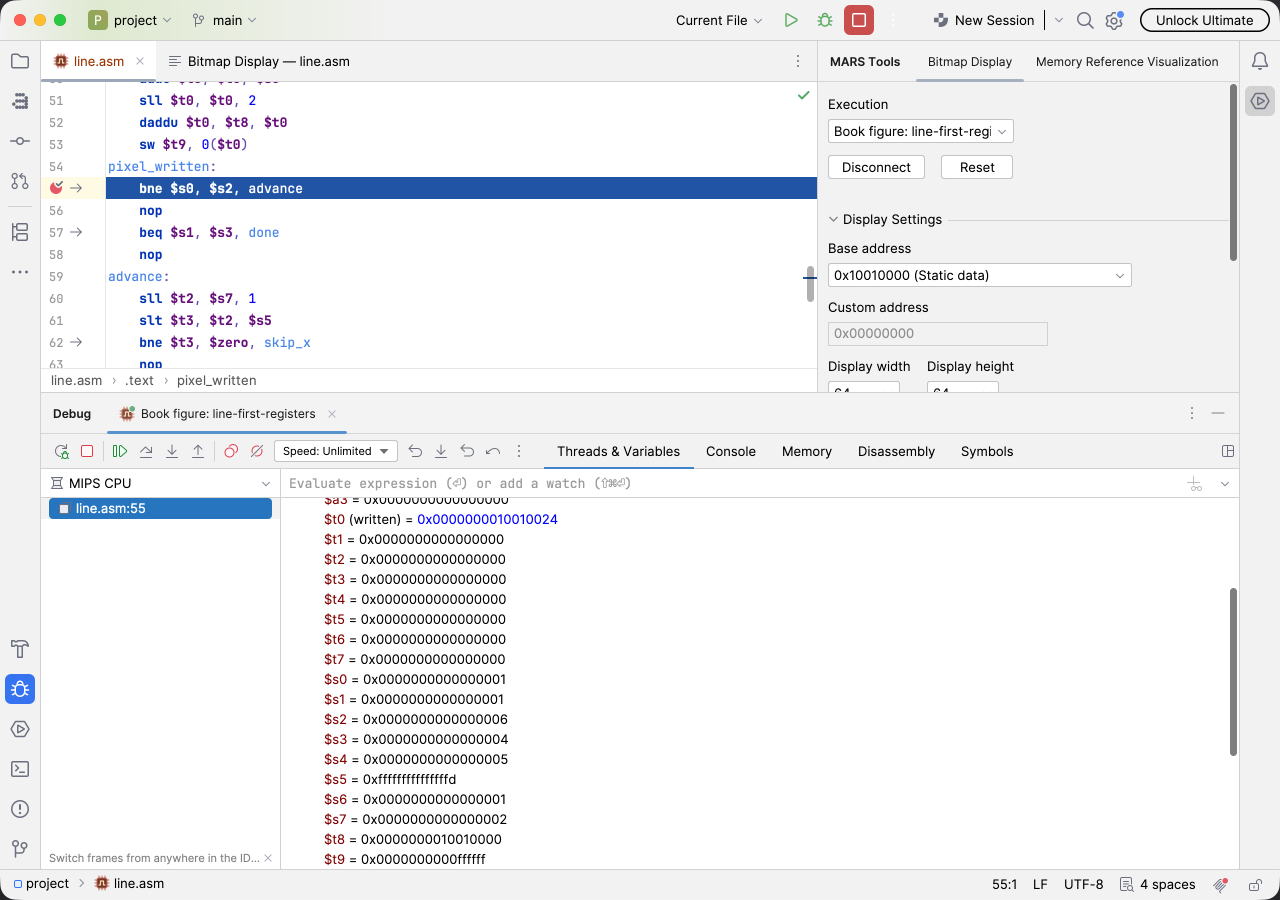
\includegraphics[width=0.4\linewidth,artifact,trim={\MARSfirststateLeft{} \MARSfirststateBottom{} \MARSfirststateRight{} \MARSfirststateTop{}},clip]{packages/007-bresenham-line/captures/f01-first/registers.png}};
    \begin{scope}[shift={(state.south west)},x={($(state.south east)-(state.south west)$)},y={($(state.north west)-(state.south west)$)}]
      \draw[black,line width=0.7pt] (0.030000000,0.018072289) rectangle (0.970000000,0.981927711);
      \node[draw=black,fill=white,circle,inner sep=1.5pt,font=\footnotesize] at ($(0.030000000,0.981927711)+(-3mm,0)$) {2};
    \end{scope}
    \node[anchor=north west,inner sep=0,font=\small\bfseries] (plot-title) at ([xshift=0.49\linewidth]state-title.north west) {Framebuffer cells};
    \node[anchor=north west,inner sep=0] (plot) at ([yshift=-1mm]plot-title.south west) {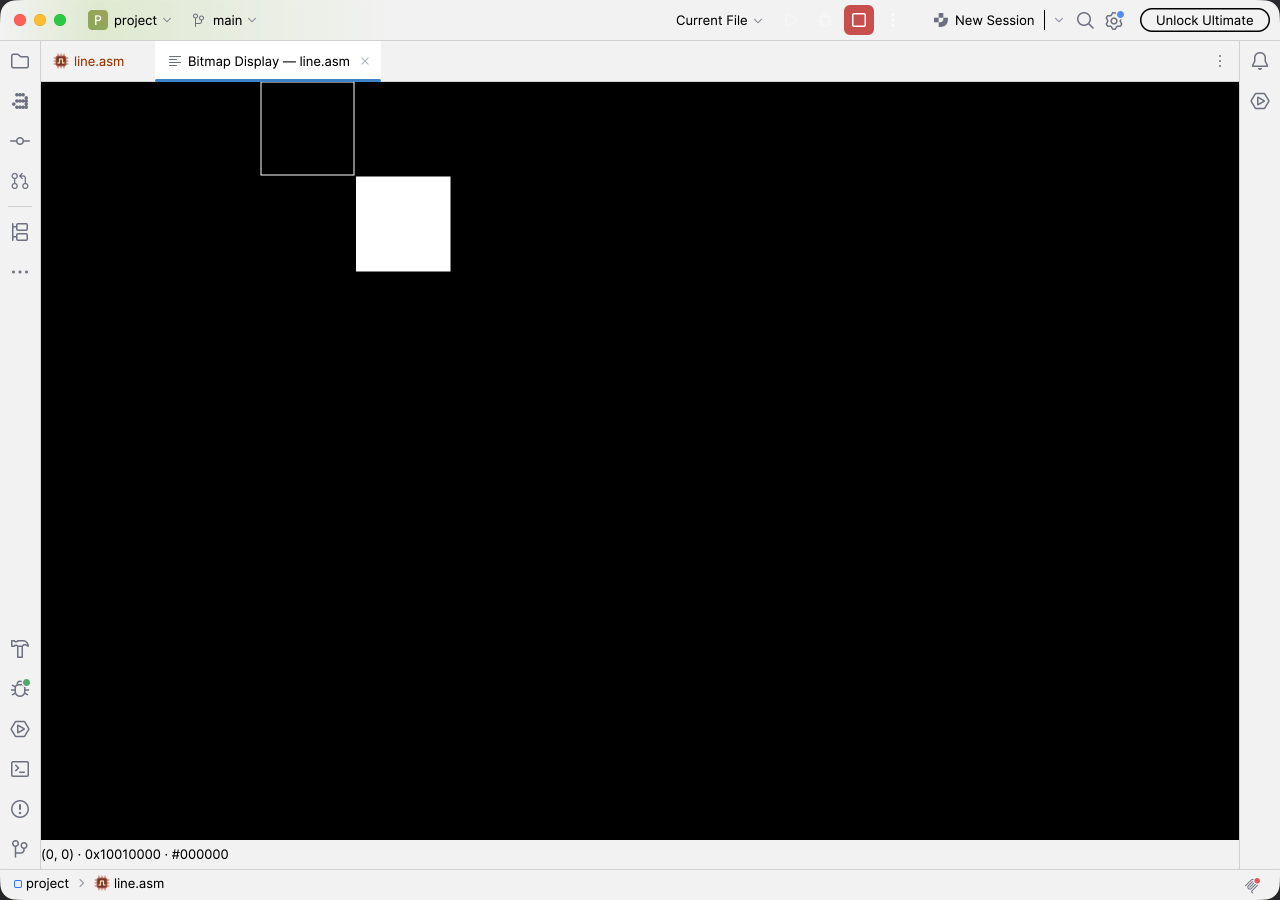
\includegraphics[width=0.32\linewidth,artifact,trim={\MARSfirstplotLeft{} \MARSfirstplotBottom{} \MARSfirstplotRight{} \MARSfirstplotTop{}},clip]{packages/007-bresenham-line/captures/f01-first/bitmap.png}};
    \begin{scope}[shift={(plot.south west)},x={($(plot.south east)-(plot.south west)$)},y={($(plot.north west)-(plot.south west)$)}]
      \draw[black,line width=0.7pt] (0.000000000,0.000000000) rectangle (1.000000000,1.000000000);
      \node[draw=black,fill=white,circle,inner sep=1.5pt,font=\footnotesize] at ($(0.000000000,1.000000000)+(-3mm,0)$) {3};
      \foreach \c in {0,...,7} {\node[anchor=north,font=\scriptsize,inner sep=0] at ({(\c+0.5)/8},-0.035) {\c}; \node[anchor=east,font=\scriptsize,inner sep=0] at (-0.025,{1-(\c+0.5)/8}) {\c};}
      \node[anchor=north,font=\scriptsize,inner sep=0] at (0.5,-0.11) {$x$}; \node[anchor=east,font=\scriptsize,inner sep=0] at (-0.10,0.5) {$y$};
    \end{scope}
  \end{tikzpicture}
  \par\smallskip
  \begin{minipage}{\linewidth}
    \small
    \begin{enumerate}
      \item The preceding \texttt{sw} has written \texttt{0x00ffffff}. The blue \texttt{bne} is the next instruction; the endpoint test and this iteration\textquotesingle s coordinate updates have not executed.
      \item \texttt{\$s0}=1 and \texttt{\$s1}=1 locate the current cell. \texttt{\$s7}=2 is the running error, initialized as $dx+dy=5+(-3)$. The constants remain $dx=5$, $dy=-3$ and $s_y=1$. The first doubled-error calculation has not executed yet.
      \item Only $(1,1)$ is white; the other 63 words retain zero. Its address is \texttt{0x10010000}+ $4(8\cdot1+1)$ = \texttt{0x10010024}. Coordinate labels outside the original image are chapter annotations. The thin native outline marks the hovered cell; white centers mark the drawn line.
    \end{enumerate}
  \end{minipage}
  \caption{The first cell has been painted. The working coordinate and running error still hold their initial values.}
  \label{capture:007-bresenham-line-f01-first}
\end{figure}
\par
